\documentclass[a4paper,norsk]{article}
\usepackage{preamble}

\begin{document}
\maketitle
\section{Exercise 1}
\subsection*{a}
LEGG TIL BILDE A PRESSURE PROFILE, BRUKES SOM REFERANSE

\subsection*{b}
According to my calculations it seems that the pressuredrop will fall beneath 50 bars after 22 years. At this time it will be necessary to install pressure support

\subsection*{c}
The fact that the contribution of liquid is neglected in this multiphase flow is due to a high Gas Oil Ratio (GOR), larger than 40000. In other words gas is dominating in the flow. The main uncertainties of this approximation is the fact that in multiphase flow the fluids contribute more to a pressuredrop  than gas(Source page 22s). Because of higher denicty So we might get a lower pressuredrop in the calculations compared to the reality. REWRITE

\subsection*{d}

\subsection*{f}
Choosing subsea compression auxiliary systems are necessary to protect the equipment and maintain an efficient productionrate.
\begin{itemize}
\item Slugging is a threat to the compressor and its interior. Installing an inlet sepparator prior to the compressor ensures that the compressor only handles clear phases, and not any solids.
\item Redusing liquid droplets in the compressor suction is essential to preserve the compressor. This is often called liquid carry over, and can be opposed by using a scrubber which is a system designed to remove these liquid dropplets from the gas stream.
The reason these liquid droplets pose a risk is at the present liquids such as water and in some sence oil is incompressible. To much incompressible vapor will damage the compressor piston as it strikes, and can overtime give extensive damage to the compressor
\item Sediments pose a risk aswell which will damage the compressor parts if they are not taken out of the gas stream. To help out reduce these sediments, chemicals can be added further down the stream to decompose the sediments before they reach the compressor inlet.
\end{itemize}

\subsection{g}
Choosing a topside or a subsea compression presents different development impacts. \\
\textbf{Project execution}
Firstly looking at production point of view a subsea solution is more efficient to produce. A topside compressor demands a platform where it can be operated, and personell to man the platform. A subsea solution demands neither, resulting in a lot of cost savings. \\
Aker solutions have also calculated a reduced CO2 emission of 60\% due to the fact that the requirement of a platform is no longer essential. 

\textbf{Operation}
Even though both solutions are made do operate for long periods of time, incidents happen. A compressor located on a platform is easier and more costefficient to maintain in operation, while a subseacomponent needed to be changed is very expensive. On the other hand a subsea solution is not exposed to harsh weather and ice found accordingly in tropic and artic areas, while a rig operation can be delayed by these factor due to equipment and personel safety. \\
Production over time will reduce the wellhead pressure, resulting in decreased flowrate in the pipes to the productionsite. Using a compressor subsea will increase productionrate by reducing the backpressure at the well as reservoir pressure is reduced over time. The pipes from the well often travels several thousand meters before they reach a topside compressor, and therefore this solution cannot give such a instant effect on the reservoir as a subsea solution.

\section*{Exercise 2}
In this section will will look at at the following flow assurance issues
\begin{itemize}
\item Slugs
\item Hydrates
\item Vibration
\end{itemize}

\subsection*{a}
\begin{figure}[h!]  
  \centering
  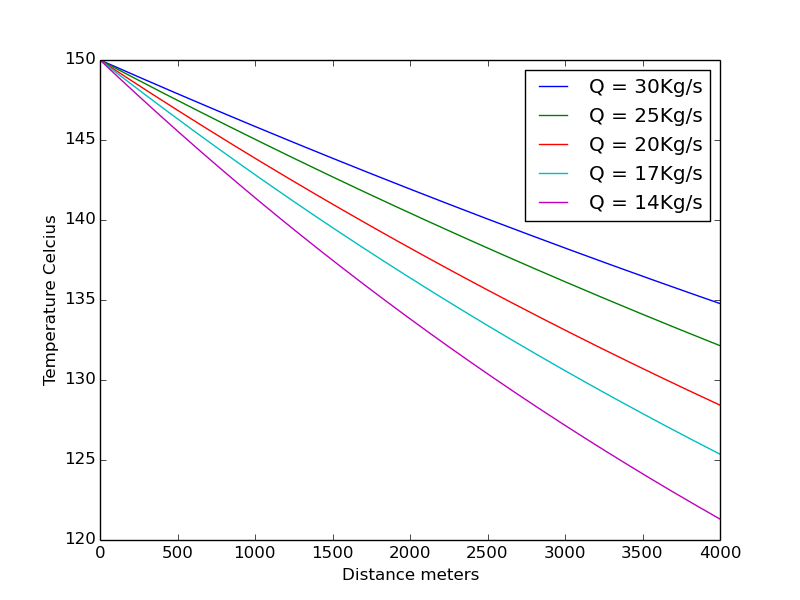
\includegraphics[scale=0.4]{wellhead.png}
  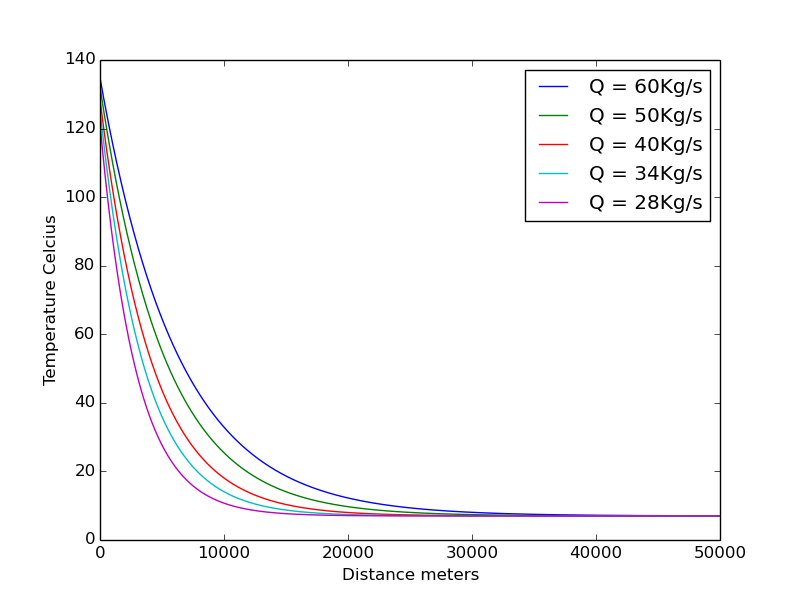
\includegraphics[scale=0.4]{shore.png}
\end{figure}
\newpage

\subsection*{b}
From our lecturenotes we know the following conditions are required to form hydrates
\begin{itemize}
\item High pressure: typically above 10-20bar at ambient temperature
\item Low temperatures: typically below 20-25 celcius
Looking at our temperatureprofile for the pipeline from the well to shore, the temperature will eventually drop beneath this critical of 20 celcius due to the long time of low seatemperature exposure. 
\end{itemize}

\subsection*{c}
From our pressureprofile for each year and corresponding temperature profile, we will unfortunately fall below the
Wax appearance temperature (WAT) presented in Figure 4 in the exercises. Ecspesially critical around 10 years, our pressure will be around 220 bar which has a peak on the WAT chart. This means that our gasflow will for a longer time be exposed to critical temperatures below WAT, resulting in a higher risk of wax deposits in the pipe. This will occur in the pipeline from the wellhead to shore. Regulary pigging of the pipe may contribute to keep the risk of wax plugs low. Other measures can be used to manipulate WAT in gas flow, such as separation at different temperatures. 

\section*{Exercise 3}
As stated in the lecturenotes hydrate management philosophy is field specific. From field to field different retarding factors influence the theoretical hydrate equilibrium conditions, but the main goal for all fields is to stay outside the hydrate formation envelope calculated by these factors. Since our system has a high GOR number, we have to focus on factors for maninly gasflow. 
\begin{itemize}
\end{itemize}

\end{document}
